\section{THD}
\label{sec:THD}
Rounding the input samples to the closest representable value according to the adopted bitwidth is a nonlinear operation that introduces distortion in the signal, producing spurious harmonics on top of the pure sinusoidal wave expected at the output of a linear filter. The relevant parameter to characterize this effect is the \textit{total harmonic distortion} (THD). The dependence of the THD on the internal bitwidth has been calculated from simulations, with the results reported in \autoref{fig:thdplot}.

%If the internal representation is the same as the one prescribed for the interface ($n_b=8$), then the THD output spectrum is as shown in figure \ref{fig:thd8bit}.
% TODO: correggere questa immagine
%\be<gin{figure}
%	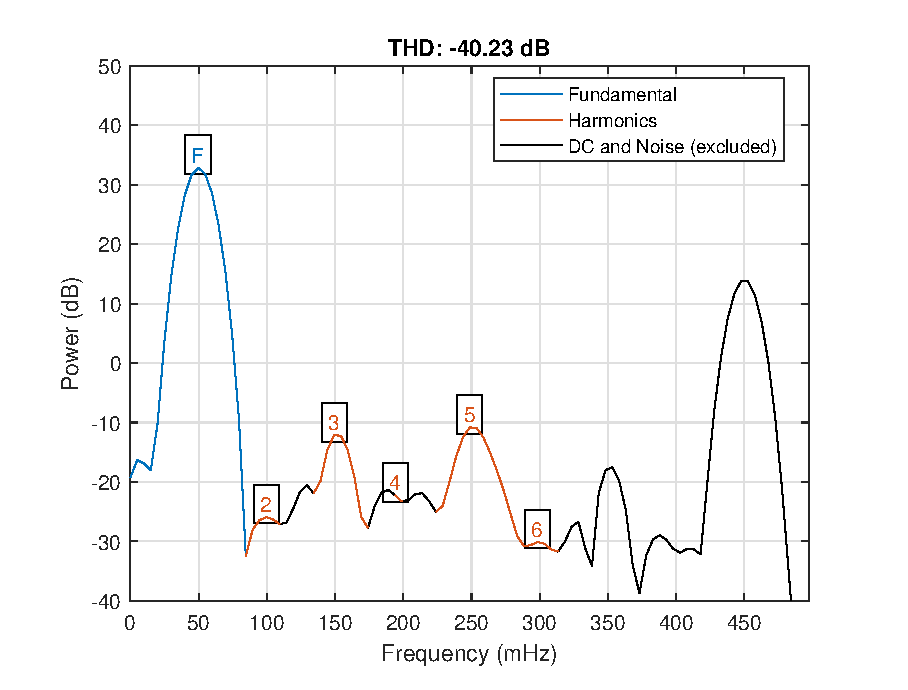
\includegraphics[width=\textwidth]{./chapter1/images/thd_with_8b.eps}
%	\caption{Spectrum and total harmonic distortion ($n_b=8$)}
%	\label{fig:thd8bit}
%\end{figure}

From these results we conclude that the smallest implementation in terms of area occupied by arithmetic operators requires $n_b=7$ in order to keep the total distortion below $\SI{-30}{dBc}$, as requested by the specifications.
